\chapter{The Morrel Family}

In a very few minutes the count reached No. 7 in the Rue Meslay. The
house was of white stone, and in a small court before it were two small
beds full of beautiful flowers. In the concierge that opened the gate
the count recognized Cocles; but as he had but one eye, and that eye
had become somewhat dim in the course of nine years, Cocles did not
recognize the count.

The carriages that drove up to the door were compelled to turn, to
avoid a fountain that played in a basin of rockwork,—an ornament that
had excited the jealousy of the whole quarter, and had gained for the
place the appellation of \textit{The Little Versailles}. It is needless to add
that there were gold and silver fish in the basin. The house, with
kitchens and cellars below, had above the ground floor, two stories and
attics. The whole of the property, consisting of an immense workshop,
two pavilions at the bottom of the garden, and the garden itself, had
been purchased by Emmanuel, who had seen at a glance that he could make
of it a profitable speculation. He had reserved the house and half the
garden, and building a wall between the garden and the workshops, had
let them upon lease with the pavilions at the bottom of the garden. So
that for a trifling sum he was as well lodged, and as perfectly shut
out from observation, as the inhabitants of the finest mansion in the
Faubourg St. Germain.

The breakfast-room was finished in oak; the salon in mahogany, and the
furnishings were of blue velvet; the bedroom was in citronwood and
green damask. There was a study for Emmanuel, who never studied, and a
music-room for Julie, who never played. The whole of the second story
was set apart for Maximilian; it was precisely similar to his sister’s
apartments, except that for the breakfast-parlor he had a
billiard-room, where he received his friends. He was superintending the
grooming of his horse, and smoking his cigar at the entrance of the
garden, when the count’s carriage stopped at the gate.

Cocles opened the gate, and Baptistin, springing from the box, inquired
whether Monsieur and Madame Herbault and Monsieur Maximilian Morrel
would see his excellency the Count of Monte Cristo.

“The Count of Monte Cristo?” cried Morrel, throwing away his cigar and
hastening to the carriage; “I should think we would see him. Ah, a
thousand thanks, count, for not having forgotten your promise.”

And the young officer shook the count’s hand so warmly, that Monte
Cristo could not be mistaken as to the sincerity of his joy, and he saw
that he had been expected with impatience, and was received with
pleasure.

“Come, come,” said Maximilian, “I will serve as your guide; such a man
as you are ought not to be introduced by a servant. My sister is in the
garden plucking the dead roses; my brother is reading his two papers,
\textit{la Presse} and \textit{les Débats}, within six steps of her; for wherever you
see Madame Herbault, you have only to look within a circle of four
yards and you will find M. Emmanuel, and ‘reciprocally,’ as they say at
the Polytechnic School.”

At the sound of their steps a young woman of twenty to five-and-twenty,
dressed in a silk morning gown, and busily engaged in plucking the dead
leaves off a noisette rose-tree, raised her head. This was Julie, who
had become, as the clerk of the house of Thomson \& French had
predicted, Madame Emmanuel Herbault. She uttered a cry of surprise at
the sight of a stranger, and Maximilian began to laugh.

“Don’t disturb yourself, Julie,” said he. “The count has only been two
or three days in Paris, but he already knows what a fashionable woman
of the Marais is, and if he does not, you will show him.”

“Ah, monsieur,” returned Julie, “it is treason in my brother to bring
you thus, but he never has any regard for his poor sister. Penelon,
Penelon!”

An old man, who was digging busily at one of the beds, stuck his spade
in the earth, and approached, cap in hand, striving to conceal a quid
of tobacco he had just thrust into his cheek. A few locks of gray
mingled with his hair, which was still thick and matted, while his
bronzed features and determined glance well suited an old sailor who
had braved the heat of the equator and the storms of the tropics.

“I think you hailed me, Mademoiselle Julie?” said he.

Penelon had still preserved the habit of calling his master’s daughter
“Mademoiselle Julie,” and had never been able to change the name to
Madame Herbault.

“Penelon,” replied Julie, “go and inform M. Emmanuel of this
gentleman’s visit, and Maximilian will conduct him to the salon.”

Then, turning to Monte Cristo,—“I hope you will permit me to leave you
for a few minutes,” continued she; and without awaiting any reply,
disappeared behind a clump of trees, and escaped to the house by a
lateral alley.

\begin{figure}[ht]
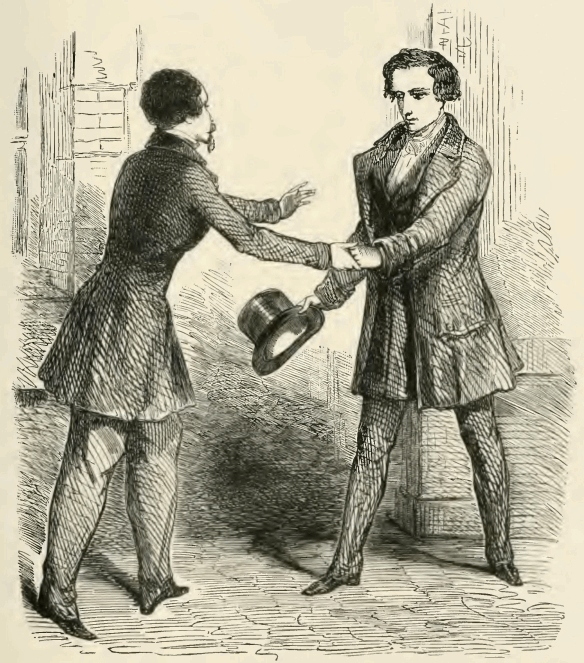
\includegraphics[width=\textwidth]{30041m.jpg}
\end{figure}

“I am sorry to see,” observed Monte Cristo to Morrel, “that I cause no
small disturbance in your house.”

“Look there,” said Maximilian, laughing; “there is her husband changing
his jacket for a coat. I assure you, you are well known in the Rue
Meslay.”

“Your family appears to be a very happy one,” said the count, as if
speaking to himself.

“Oh, yes, I assure you, count, they want nothing that can render them
happy; they are young and cheerful, they are tenderly attached to each
other, and with twenty-five thousand francs a year they fancy
themselves as rich as Rothschild.”

“Five-and-twenty thousand francs is not a large sum, however,” replied
Monte Cristo, with a tone so sweet and gentle, that it went to
Maximilian’s heart like the voice of a father; “but they will not be
content with that. Your brother-in-law is a barrister? a doctor?”

“He was a merchant, monsieur, and had succeeded to the business of my
poor father. M. Morrel, at his death, left 500,000 francs, which were
divided between my sister and myself, for we were his only children.
Her husband, who, when he married her, had no other patrimony than his
noble probity, his first-rate ability, and his spotless reputation,
wished to possess as much as his wife. He labored and toiled until he
had amassed 250,000 francs; six years sufficed to achieve this object.
Oh, I assure you, sir, it was a touching spectacle to see these young
creatures, destined by their talents for higher stations, toiling
together, and through their unwillingness to change any of the customs
of their paternal house, taking six years to accomplish what less
scrupulous people would have effected in two or three. Marseilles
resounded with their well-earned praises. At last, one day, Emmanuel
came to his wife, who had just finished making up the accounts.

“‘Julie,’ said he to her, ‘Cocles has just given me the last rouleau of
a hundred francs; that completes the 250,000 francs we had fixed as the
limits of our gains. Can you content yourself with the small fortune
which we shall possess for the future? Listen to me. Our house
transacts business to the amount of a million a year, from which we
derive an income of 40,000 francs. We can dispose of the business, if
we please, in an hour, for I have received a letter from M. Delaunay,
in which he offers to purchase the good-will of the house, to unite
with his own, for 300,000 francs. Advise me what I had better do.’

“‘Emmanuel,’ returned my sister, ‘the house of Morrel can only be
carried on by a Morrel. Is it not worth 300,000 francs to save our
father’s name from the chances of evil fortune and failure?’

“‘I thought so,’ replied Emmanuel; ‘but I wished to have your advice.’

“‘This is my counsel:—Our accounts are made up and our bills paid; all
we have to do is to stop the issue of any more, and close our office.’

“This was done instantly. It was three o’clock; at a quarter past, a
merchant presented himself to insure two ships; it was a clear profit
of 15,000 francs.

“‘Monsieur,’ said Emmanuel, ‘have the goodness to address yourself to
M. Delaunay. We have quitted business.’

“‘How long?’ inquired the astonished merchant.

\begin{figure}[ht]
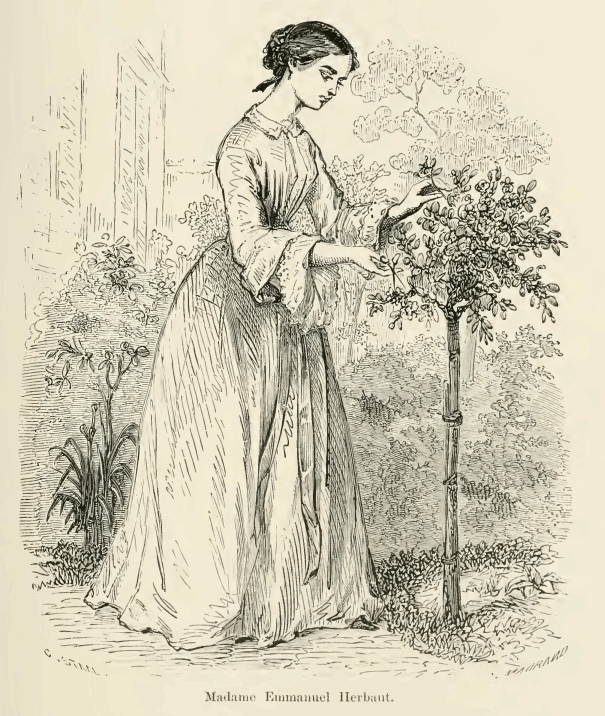
\includegraphics[width=\textwidth]{30043m.jpg}
\end{figure}

“‘A quarter of an hour,’ was the reply.

“And this is the reason, monsieur,” continued Maximilian, “of my sister
and brother-in-law having only 25,000 francs a year.”

Maximilian had scarcely finished his story, during which the count’s
heart had swelled within him, when Emmanuel entered wearing a hat and
coat. He saluted the count with the air of a man who is aware of the
rank of his guest; then, after having led Monte Cristo around the
little garden, he returned to the house.

A large vase of Japan porcelain, filled with flowers that loaded the
air with their perfume, stood in the salon. Julie, suitably dressed,
and her hair arranged (she had accomplished this feat in less than ten
minutes), received the count on his entrance. The songs of the birds
were heard in an aviary hard by, and the branches of laburnums and rose
acacias formed an exquisite framework to the blue velvet curtains.
Everything in this charming retreat, from the warble of the birds to
the smile of the mistress, breathed tranquillity and repose.

The count had felt the influence of this happiness from the moment he
entered the house, and he remained silent and pensive, forgetting that
he was expected to renew the conversation, which had ceased after the
first salutations had been exchanged. The silence became almost painful
when, by a violent effort, tearing himself from his pleasing reverie:

“Madame,” said he at length, “I pray you to excuse my emotion, which
must astonish you who are only accustomed to the happiness I meet here;
but contentment is so new a sight to me, that I could never be weary of
looking at yourself and your husband.”

“We are very happy, monsieur,” replied Julie; “but we have also known
unhappiness, and few have ever undergone more bitter sufferings than
ourselves.”

The count’s features displayed an expression of the most intense
curiosity.

“Oh, all this is a family history, as Château-Renaud told you the other
day,” observed Maximilian. “This humble picture would have but little
interest for you, accustomed as you are to behold the pleasures and the
misfortunes of the wealthy and industrious; but such as we are, we have
experienced bitter sorrows.”

“And God has poured balm into your wounds, as he does into those of all
who are in affliction?” said Monte Cristo inquiringly.

“Yes, count,” returned Julie, “we may indeed say he has, for he has
done for us what he grants only to his chosen; he sent us one of his
angels.”

The count’s cheeks became scarlet, and he coughed, in order to have an
excuse for putting his handkerchief to his mouth.

“Those born to wealth, and who have the means of gratifying every
wish,” said Emmanuel, “know not what is the real happiness of life,
just as those who have been tossed on the stormy waters of the ocean on
a few frail planks can alone realize the blessings of fair weather.”

Monte Cristo rose, and without making any answer (for the tremulousness
of his voice would have betrayed his emotion) walked up and down the
apartment with a slow step.

“Our magnificence makes you smile, count,” said Maximilian, who had
followed him with his eyes.

“No, no,” returned Monte Cristo, pale as death, pressing one hand on
his heart to still its throbbings, while with the other he pointed to a
crystal cover, beneath which a silken purse lay on a black velvet
cushion. “I was wondering what could be the significance of this purse,
with the paper at one end and the large diamond at the other.”

“Count,” replied Maximilian, with an air of gravity, “those are our
most precious family treasures.”

“The stone seems very brilliant,” answered the count.

“Oh, my brother does not allude to its value, although it has been
estimated at 100,000 francs; he means, that the articles contained in
this purse are the relics of the angel I spoke of just now.”

“This I do not comprehend; and yet I may not ask for an explanation,
madame,” replied Monte Cristo bowing. “Pardon me, I had no intention of
committing an indiscretion.”

“Indiscretion,—oh, you make us happy by giving us an excuse for
expatiating on this subject. If we wanted to conceal the noble action
this purse commemorates, we should not expose it thus to view. Oh,
would we could relate it everywhere, and to everyone, so that the
emotion of our unknown benefactor might reveal his presence.”

“Ah, really,” said Monte Cristo in a half-stifled voice.

“Monsieur,” returned Maximilian, raising the glass cover, and
respectfully kissing the silken purse, “this has touched the hand of a
man who saved my father from suicide, us from ruin, and our name from
shame and disgrace,—a man by whose matchless benevolence we poor
children, doomed to want and wretchedness, can at present hear everyone
envying our happy lot. This letter” (as he spoke, Maximilian drew a
letter from the purse and gave it to the count)—“this letter was
written by him the day that my father had taken a desperate resolution,
and this diamond was given by the generous unknown to my sister as her
dowry.”

Monte Cristo opened the letter, and read it with an indescribable
feeling of delight. It was the letter written (as our readers know) to
Julie, and signed “Sinbad the Sailor.”

“Unknown you say, is the man who rendered you this service—unknown to
you?”

“Yes; we have never had the happiness of pressing his hand,” continued
Maximilian. “We have supplicated Heaven in vain to grant us this favor,
but the whole affair has had a mysterious meaning that we cannot
comprehend—we have been guided by an invisible hand,—a hand as powerful
as that of an enchanter.”

“Oh,” cried Julie, “I have not lost all hope of some day kissing that
hand, as I now kiss the purse which he has touched. Four years ago,
Penelon was at Trieste—Penelon, count, is the old sailor you saw in the
garden, and who, from quartermaster, has become gardener—Penelon, when
he was at Trieste, saw on the quay an Englishman, who was on the point
of embarking on board a yacht, and he recognized him as the person who
called on my father the fifth of June, 1829, and who wrote me this
letter on the fifth of September. He felt convinced of his identity,
but he did not venture to address him.”

“An Englishman,” said Monte Cristo, who grew uneasy at the attention
with which Julie looked at him. “An Englishman you say?”

“Yes,” replied Maximilian, “an Englishman, who represented himself as
the confidential clerk of the house of Thomson \& French, at Rome. It
was this that made me start when you said the other day, at M. de
Morcerf’s, that Messrs. Thomson \& French were your bankers. That
happened, as I told you, in 1829. For God’s sake, tell me, did you know
this Englishman?”

“But you tell me, also, that the house of Thomson \& French have
constantly denied having rendered you this service?”

“Yes.”

“Then is it not probable that this Englishman may be someone who,
grateful for a kindness your father had shown him, and which he himself
had forgotten, has taken this method of requiting the obligation?”

“Everything is possible in this affair, even a miracle.”

“What was his name?” asked Monte Cristo.

“He gave no other name,” answered Julie, looking earnestly at the
count, “than that at the end of his letter—‘Sinbad the Sailor.’”

“Which is evidently not his real name, but a fictitious one.”

Then, noticing that Julie was struck with the sound of his voice:

“Tell me,” continued he, “was he not about my height, perhaps a little
taller, with his chin imprisoned, as it were, in a high cravat; his
coat closely buttoned up, and constantly taking out his pencil?”

“Oh, do you then know him?” cried Julie, whose eyes sparkled with joy.

“No,” returned Monte Cristo “I only guessed. I knew a Lord Wilmore, who
was constantly doing actions of this kind.”

“Without revealing himself?”

“He was an eccentric being, and did not believe in the existence of
gratitude.”

“Oh, Heaven,” exclaimed Julie, clasping her hands, “in what did he
believe, then?”

\begin{figure}[ht]
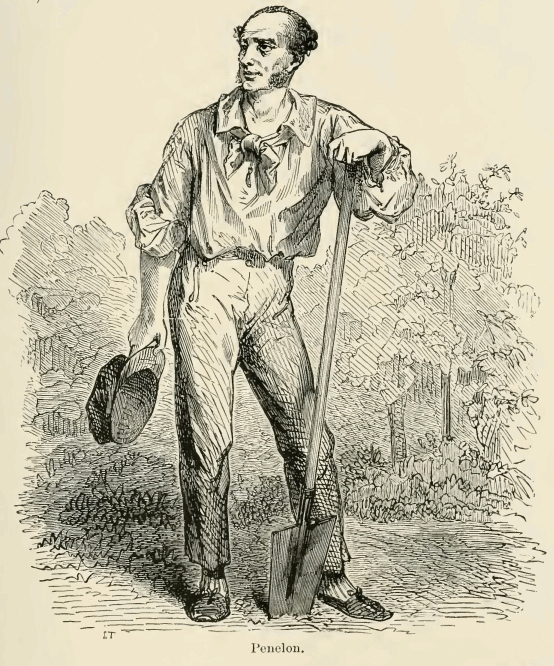
\includegraphics[width=\textwidth]{30047m.jpg}
\end{figure}

“He did not credit it at the period which I knew him,” said Monte
Cristo, touched to the heart by the accents of Julie’s voice; “but,
perhaps, since then he has had proofs that gratitude does exist.”

“And do you know this gentleman, monsieur?” inquired Emmanuel.

“Oh, if you do know him,” cried Julie, “can you tell us where he
is—where we can find him? Maximilian—Emmanuel—if we do but discover
him, he must believe in the gratitude of the heart!”

Monte Cristo felt tears start into his eyes, and he again walked
hastily up and down the room.

“In the name of Heaven,” said Maximilian, “if you know anything of him,
tell us what it is.”

“Alas,” cried Monte Cristo, striving to repress his emotion, “if Lord
Wilmore was your unknown benefactor, I fear you will never see him
again. I parted from him two years ago at Palermo, and he was then on
the point of setting out for the most remote regions; so that I fear he
will never return.”

“Oh, monsieur, this is cruel of you,” said Julie, much affected; and
the young lady’s eyes swam with tears.

“Madame,” replied Monte Cristo gravely, and gazing earnestly on the two
liquid pearls that trickled down Julie’s cheeks, “had Lord Wilmore seen
what I now see, he would become attached to life, for the tears you
shed would reconcile him to mankind;” and he held out his hand to
Julie, who gave him hers, carried away by the look and accent of the
count.

“But,” continued she, “Lord Wilmore had a family or friends, he must
have known someone, can we not——”

“Oh, it is useless to inquire,” returned the count; “perhaps, after
all, he was not the man you seek for. He was my friend: he had no
secrets from me, and if this had been so he would have confided in me.”

“And he told you nothing?”

“Not a word.”

“Nothing that would lead you to suppose?”

“Nothing.”

“And yet you spoke of him at once.”

“Ah, in such a case one supposes——”

“Sister, sister,” said Maximilian, coming to the count’s aid, “monsieur
is quite right. Recollect what our excellent father so often told us,
‘It was no Englishman that thus saved us.’”

Monte Cristo started. “What did your father tell you, M. Morrel?” said
he eagerly.

“My father thought that this action had been miraculously performed—he
believed that a benefactor had arisen from the grave to save us. Oh, it
was a touching superstition, monsieur, and although I did not myself
believe it, I would not for the world have destroyed my father’s faith.
How often did he muse over it and pronounce the name of a dear friend—a
friend lost to him forever; and on his death-bed, when the near
approach of eternity seemed to have illumined his mind with
supernatural light, this thought, which had until then been but a
doubt, became a conviction, and his last words were, ‘Maximilian, it
was Edmond Dantès!’”

At these words the count’s paleness, which had for some time been
increasing, became alarming; he could not speak; he looked at his watch
like a man who has forgotten the hour, said a few hurried words to
Madame Herbault, and pressing the hands of Emmanuel and
Maximilian,—“Madame,” said he, “I trust you will allow me to visit you
occasionally; I value your friendship, and feel grateful to you for
your welcome, for this is the first time for many years that I have
thus yielded to my feelings;” and he hastily quitted the apartment.

“This Count of Monte Cristo is a strange man,” said Emmanuel.

“Yes,” answered Maximilian, “but I feel sure he has an excellent heart,
and that he likes us.”

“His voice went to my heart,” observed Julie; “and two or three times I
fancied that I had heard it before.”
